% !TeX root = ./Report-Body.tex
\chapter{Example Relaxation Rate Calculations} \label{chapB}
\allowdisplaybreaks

\begin{appendixtext}
In this appendix, I illustrate some explicit calculations of a few relaxation rates, for an IS dipolar spin system, undergoing spherical isotropic motion. This is one of the simplest possible relaxation rate calculations that can be done, as only a single interaction is acting. As the number of spins in the spin-system increases, as well as the number of relaxation mechanisms involved, the scale of the calculation drastically rises to the point where it is not feasible to show the calculation in a detailed fashion.\\

\section{Setting Up The Calculation} \label{secB.1}
As only a single mechanism is inducing relaxation in our system of interest, the summations over $i_1$ and $i_2$ are not necessary. As well as this, it isn't necessary to perform a rotation into the molecular frame when a single interaction tensor is present. Therefore, \ref{SpherOpElement} reduces to: 
\begin{equation}
\label{eqB.1}
\Gamma_{rs} = \frac{6}{5} d_{\text{IS}}^2 \sum \limits_{k = -2}^2 \sum \limits_{n_1} \sum \limits_{n_2} \frac{\bra{\hat{\rho}_s} \ket{\comm{\hat{T}_{k, n_1}^{(2) \dagger}}{\comm{\hat{T}_{k,n_2}^{(2)}}{\hat{\rho}_r}}} J(\omega_{k,n_2})}{\sqrt{\bra{\hat{\rho}_r} \ket{\hat{\rho}_r} \bra{\hat{\rho}_s} \ket{\hat{\rho}_s}}}
\end{equation}
where the dipolar interaction constant, $d_{\text{IS}}$, is defined in \ref{DipConst} and expressions for the operators $\hat{T}_{k,n}^{(2)}$ are given in Table \ref{SphericalOperators}. A total of 19 terms therefore exist in this summation. Calculations of each of these terms are shown below, first for $r=s=\hat{I}_z$ and then for $r=s=\hat{I}^+$. The results of these calculations give the longitudinal and transverse relaxation rates of spin I, respectively.
\section{Longitudinal Relaxation} \label{secB.2}
First, we will consider the longitudinal relaxation rate of spin I, which is determined by setting $\hat{\rho}_r = \hat{\rho}_s = \hat{I}_z$. By noting that $\bra{\hat{I}_z} \ket{\hat{I}_z} = 1$, this rate is given by:
\begin{equation}
\label{eqB.2}
\Gamma_{1,\text{I}} = \frac{6}{5} d_{\text{IS}}^2 \sum \limits_{k = -2}^2 \sum \limits_{n_1} \sum \limits_{n_2} \bra{\hat{I}_z} \ket{\comm{\hat{T}_{k, n_1}^{(2) \dagger}}{\comm{\hat{T}_{k,n_2}^{(2)}}{\hat{I}_z}}} J(\omega_{k,n_2})
\end{equation}
where $J(\omega_{k,n_2}) = \frac{\tau_{\text{c}}}{1 + \omega_{k,n_2}^2\tau_{\text{c}}^2}$.
\subsection{Calculating individual terms} \label{subsecB.2.1}
\subsubsection{$\mathbf{k = -2}$}
$n_1 = n_2 = 1$:
\begin{align*}
&\frac{6}{5} d_{\text{IS}}^2 \bra{\hat{I}_z} \ket{\comm{\hat{T}_{-2, 1}^{(2) \dagger}}{\comm{\hat{T}_{-2,1}^{(2)}}{\hat{I}_z}}} J(\omega_{-2,1}) = \frac{3}{10} d_{\text{IS}}^2 \bra{\hat{I}_z} \ket{\comm{\hat{I}^+ \hat{S}^+}{\comm{\hat{I}^- \hat{S}^-}{\hat{I}_z}}} J(-\omega_{\text{I}} - \omega_{\text{S}}) \\
&= \frac{3}{10} d_{\text{IS}}^2 \bra{\hat{I}_z} \ket{\comm{\hat{I}^+ \hat{S}^+}{\hat{I}^- \hat{S}^-}} J(-\omega_{\text{I}} - \omega_{\text{S}}) = \frac{3}{10} d_{\text{IS}}^2 \bra{\hat{I}_z} \ket{\hat{I}_z + \hat{S}_z} J(-\omega_{\text{I}} - \omega_{\text{S}}) \\
& = \underline{\frac{3}{10} d_{\text{IS}}^2 J(-\omega_{\text{I}} - \omega_{\text{S}})}
\end{align*}
\subsubsection{$\mathbf{k = -1}$}
$n_1 = n_2 = 1$:
\begin{align*}
&\frac{6}{5} d_{\text{IS}}^2 \bra{\hat{I}_z} \ket{\comm{\hat{T}_{-1, 1}^{(2) \dagger}}{\comm{\hat{T}_{-1,1}^{(2)}}{\hat{I}_z}}} J(\omega_{-1,1}) = \frac{3}{10} d_{\text{IS}}^2 \bra{\hat{I}_z} \ket{\comm{\hat{I}_z \hat{S}^+}{\comm{\hat{I}_z \hat{S}^-}{\hat{I}_z}}} J(- \omega_{\text{S}}) \\
&= 0
\end{align*}
$n_1 = 1, n_2 = 2$:
\begin{align*}
&\frac{6}{5} d_{\text{IS}}^2 \bra{\hat{I}_z} \ket{\comm{\hat{T}_{-1, 1}^{(2) \dagger}}{\comm{\hat{T}_{-1,2}^{(2)}}{\hat{I}_z}}} J(\omega_{-1,2}) = \frac{3}{10} d_{\text{IS}}^2 \bra{\hat{I}_z} \ket{\comm{\hat{I}_z \hat{S}^+}{\comm{\hat{I}^- \hat{S}_z}{\hat{I}_z}}} J(- \omega_{\text{I}}) \\
&= \frac{3}{10} d_{\text{IS}}^2 \bra{\hat{I}_z} \ket{\comm{\hat{I}_z \hat{S}^+}{\hat{I}^- \hat{S}_z}} J(- \omega_{\text{I}}) =  \frac{3}{10} d_{\text{IS}}^2 \bra{\hat{I}_z} \ket{\hat{I}^- \hat{S}^+} J(- \omega_{\text{I}}) \\
& = 0
\end{align*}
$n_1 = 2, n_2 = 1$:
\begin{align*}
&\frac{6}{5} d_{\text{IS}}^2 \bra{\hat{I}_z} \ket{\comm{\hat{T}_{-1, 2}^{(2) \dagger}}{\comm{\hat{T}_{-1,1}^{(2)}}{\hat{I}_z}}} J(\omega_{-1,1}) = \frac{3}{10} d_{\text{IS}}^2 \bra{\hat{I}_z} \ket{\comm{\hat{I}^+ \hat{S}_z}{\comm{\hat{I}_z \hat{S}^-}{\hat{I}_z}}} J(- \omega_{\text{S}}) \\
&= 0
\end{align*}
$n_1 = n_2 = 2$:
\begin{align*}
&\frac{6}{5} d_{\text{IS}}^2 \bra{\hat{I}_z} \ket{\comm{\hat{T}_{-1, 2}^{(2) \dagger}}{\comm{\hat{T}_{-1,2}^{(2)}}{\hat{I}_z}}} J(\omega_{-1,2}) = \frac{3}{10} d_{\text{IS}}^2 \bra{\hat{I}_z} \ket{\comm{\hat{I}^+ \hat{S}_z}{\comm{\hat{I}^- \hat{S}_z}{\hat{I}_z}}} J(- \omega_{\text{I}}) \\
&= \frac{3}{10} d_{\text{IS}}^2 \bra{\hat{I}_z} \ket{\comm{\hat{I}^+ \hat{S}_z}{\hat{I}^- \hat{S}_z}} J(- \omega_{\text{I}}) = \frac{3}{10} d_{\text{IS}}^2 \bra{\hat{I}_z} \ket{2 \hat{I}_z \hat{S}_z^2} J(- \omega_{\text{I}}) \\
&= \frac{3}{20} d_{\text{IS}}^2 \bra{\hat{I}_z} \ket{\hat{I}_z} J(- \omega_{\text{I}}) = \underline{\frac{3}{20} d_{\text{IS}}^2 J(- \omega_{\text{I}})}
\end{align*}
\subsubsection{$\mathbf{k = 0}$}
$n_1 = 1, n_2 = 1$:
\begin{align*}
&\frac{6}{5} d_{\text{IS}}^2 \bra{\hat{I}_z} \ket{\comm{\hat{T}_{0, 1}^{(2) \dagger}}{\comm{\hat{T}_{0,1}^{(2)}}{\hat{I}_z}}} J(\omega_{0,1}) = \frac{4}{5} d_{\text{IS}}^2 \bra{\hat{I}_z} \ket{\comm{\hat{I}_z \hat{S}_z}{\comm{\hat{I}_z \hat{S}_z}{\hat{I}_z}}} J(0) \\
&= 0
\end{align*}
$n_1 = 1, n_2 = 2$:
\begin{align*}
&\frac{6}{5} d_{\text{IS}}^2 \bra{\hat{I}_z} \ket{\comm{\hat{T}_{0,1}^{(2) \dagger}}{\comm{\hat{T}_{0,2}^{(2)}}{\hat{I}_z}}} J(\omega_{0,2}) = -\frac{1}{5} d_{\text{IS}}^2 \bra{\hat{I}_z} \ket{\comm{\hat{I}_z \hat{S}_z}{\comm{\hat{I}^+ \hat{S}^-}{\hat{I}_z}}} J(\omega_{\text{I}} - \omega_{\text{S}}) \\
&= \frac{1}{5} d_{\text{IS}}^2 \bra{\hat{I}_z} \ket{\comm{\hat{I}_z \hat{S}_z}{\hat{I}^+ \hat{S}^-}} J(\omega_{\text{I}} - \omega_{\text{S}}) = -\frac{1}{5} d_{\text{IS}}^2 \bra{\hat{I}_z} \ket{\hat{I}^+ \hat{S}^-} J(\omega_{\text{I}} - \omega_{\text{S}}) \\
& = 0
\end{align*}
$n_1 = 1, n_2 = 3$:
\begin{align*}
&\frac{6}{5} d_{\text{IS}}^2 \bra{\hat{I}_z} \ket{\comm{\hat{T}_{0,1}^{(2) \dagger}}{\comm{\hat{T}_{0,3}^{(2)}}{\hat{I}_z}}} J(\omega_{0,3}) = -\frac{1}{5} d_{\text{IS}}^2 \bra{\hat{I}_z} \ket{\comm{\hat{I}_z \hat{S}_z}{\comm{\hat{I}^- \hat{S}^+}{\hat{I}_z}}} J(\omega_{\text{S}} - \omega_{\text{I}}) \\
&= -\frac{1}{5} d_{\text{IS}}^2 \bra{\hat{I}_z} \ket{\comm{\hat{I}_z \hat{S}_z}{\hat{I}^- \hat{S}^+}} J(\omega_{\text{S}} - \omega_{\text{I}}) = \frac{1}{5} d_{\text{IS}}^2 \bra{\hat{I}_z} \ket{\hat{I}^- \hat{S}^+} J(\omega_{\text{S}} - \omega_{\text{I}}) \\
&= 0
\end{align*}
$n_1 = 2, n_2 = 1$:
\begin{align*}
&\frac{6}{5} d_{\text{IS}}^2 \bra{\hat{I}_z} \ket{\comm{\hat{T}_{0,2}^{(2) \dagger}}{\comm{\hat{T}_{0,1}^{(2)}}{\hat{I}_z}}} J(\omega_{0,1}) = -\frac{1}{5} d_{\text{IS}}^2 \bra{\hat{I}_z} \ket{\comm{\hat{I}^- \hat{S}^+}{\comm{\hat{I}_z \hat{S}_z}{\hat{I}_z}}} J(0) \\
&= 0
\end{align*}
$n_1 = 2, n_2 = 2$:
\begin{align*}
&\frac{6}{5} d_{\text{IS}}^2 \bra{\hat{I}_z} \ket{\comm{\hat{T}_{0, 2}^{(2) \dagger}}{\comm{\hat{T}_{0,2}^{(2)}}{\hat{I}_z}}} J(\omega_{0,2}) = \frac{1}{20} d_{\text{IS}}^2 \bra{\hat{I}_z} \ket{\comm{\hat{I}^- \hat{S}^+}{\comm{\hat{I}^+ \hat{S}^-}{\hat{I}_z}}} J(\omega_{\text{I}} - \omega_{\text{S}}) \\
&= -\frac{1}{20} d_{\text{IS}}^2 \bra{\hat{I}_z} \ket{\comm{\hat{I}^- \hat{S}^+}{\hat{I}^+ \hat{S}^-}} J(\omega_{\text{I}} - \omega_{\text{S}}) = -\frac{1}{20} d_{\text{IS}}^2 \bra{\hat{I}_z} \ket{\hat{S}_z - \hat{I}_z} J(\omega_{\text{I}} - \omega_{\text{S}}) \\
& = \underline{\frac{1}{20} d_{\text{IS}}^2 J(\omega_{\text{I}} - \omega_{\text{S}})}
\end{align*}
$n_1 = 2, n_2 = 3$:
\begin{align*}
&\frac{6}{5} d_{\text{IS}}^2 \bra{\hat{I}_z} \ket{\comm{\hat{T}_{0,2}^{(2) \dagger}}{\comm{\hat{T}_{0,3}^{(2)}}{\hat{I}_z}}} J(\omega_{0,3}) = \frac{1}{20} d_{\text{IS}}^2 \bra{\hat{I}_z} \ket{\comm{\hat{I}^- \hat{S}^+}{\comm{\hat{I}^- \hat{S}^+}{\hat{I}_z}}} J(\omega_{\text{S}} - \omega_{\text{I}}) \\
&= \frac{1}{20} d_{\text{IS}}^2 \bra{\hat{I}_z} \ket{\comm{\hat{I}^- \hat{S}^+}{\hat{I}^- \hat{S}^+}} J(\omega_{\text{S}} - \omega_{\text{I}}) = 0
\end{align*}
$n_1 = 3, n_2 = 1$:
\begin{align*}
&\frac{6}{5} d_{\text{IS}}^2 \bra{\hat{I}_z} \ket{\comm{\hat{T}_{0,3}^{(2) \dagger}}{\comm{\hat{T}_{0,1}^{(2)}}{\hat{I}_z}}} J(\omega_{0,1}) = -\frac{1}{5} d_{\text{IS}}^2 \bra{\hat{I}_z} \ket{\comm{\hat{I}^+ \hat{S}^-}{\comm{\hat{I}_z \hat{S}_z}{\hat{I}_z}}} J(0) \\
&= 0
\end{align*}
$n_1 = 3, n_2 = 2$:
\begin{align*}
&\frac{6}{5} d_{\text{IS}}^2 \bra{\hat{I}_z} \ket{\comm{\hat{T}_{0,3}^{(2) \dagger}}{\comm{\hat{T}_{0,2}^{(2)}}{\hat{I}_z}}} J(\omega_{0,2}) = \frac{1}{20} d_{\text{IS}}^2 \bra{\hat{I}_z} \ket{\comm{\hat{I}^+ \hat{S}^-}{\comm{\hat{I}^+ \hat{S}^-}{\hat{I}_z}}} J(\omega_{\text{I}} - \omega_{\text{S}}) \\
&= -\frac{1}{20} d_{\text{IS}}^2 \bra{\hat{I}_z} \ket{\comm{\hat{I}^+ \hat{S}^-}{\hat{I}^+ \hat{S}^-}} J(\omega_{\text{I}} - \omega_{\text{S}}) = 0
\end{align*}
$n_1 = 3, n_2 = 3$:
\begin{align*}
&\frac{6}{5} d_{\text{IS}}^2 \bra{\hat{I}_z} \ket{\comm{\hat{T}_{0,3}^{(2) \dagger}}{\comm{\hat{T}_{0,3}^{(2)}}{\hat{I}_z}}} J(\omega_{0,3}) = \frac{1}{20} d_{\text{IS}}^2 \bra{\hat{I}_z} \ket{\comm{\hat{I}^+ \hat{S}^-}{\comm{\hat{I}^- \hat{S}^+}{\hat{I}_z}}} J(\omega_{\text{S}} - \omega_{\text{I}}) \\
&= \frac{1}{20} d_{\text{IS}}^2 \bra{\hat{I}_z} \ket{\comm{\hat{I}^+ \hat{S}^-}{\hat{I}^- \hat{S}^+}} J(\omega_{\text{S}} - \omega_{\text{I}}) = \frac{1}{20} d_{\text{IS}}^2 \bra{\hat{I}_z} \ket{\hat{I}_z - \hat{S}_z} J(\omega_{\text{S}} - \omega_{\text{I}}) \\
&= \underline{\frac{1}{20} d_{\text{IS}}^2 J(\omega_{\text{S}} - \omega_{\text{I}})}
\end{align*}
\subsubsection{$\mathbf{k = 1}$}
$n_1 = n_2 = 1$:
\begin{align*}
&\frac{6}{5} d_{\text{IS}}^2 \bra{\hat{I}_z} \ket{\comm{\hat{T}_{1, 1}^{(2) \dagger}}{\comm{\hat{T}_{1,1}^{(2)}}{\hat{I}_z}}} J(\omega_{1,1}) = \frac{3}{10} d_{\text{IS}}^2 \bra{\hat{I}_z} \ket{\comm{\hat{I}_z \hat{S}^+}{\comm{\hat{I}_z \hat{S}^+}{\hat{I}_z}}} J(\omega_{\text{S}}) \\
&= 0
\end{align*}
$n_1 = 1, n_2 = 2$:
\begin{align*}
&\frac{6}{5} d_{\text{IS}}^2 \bra{\hat{I}_z} \ket{\comm{\hat{T}_{1, 1}^{(2) \dagger}}{\comm{\hat{T}_{1,2}^{(2)}}{\hat{I}_z}}} J(\omega_{1,2}) = \frac{3}{10} d_{\text{IS}}^2 \bra{\hat{I}_z} \ket{\comm{\hat{I}_z \hat{S}^-}{\comm{\hat{I}^+ \hat{S}_z}{\hat{I}_z}}} J(\omega_{\text{I}}) \\
&= -\frac{3}{10} d_{\text{IS}}^2 \bra{\hat{I}_z} \ket{\comm{\hat{I}_z \hat{S}^-}{\hat{I}^+ \hat{S}_z}} J(\omega_{\text{I}}) = -\frac{3}{10} d_{\text{IS}}^2 \bra{\hat{I}_z} \ket{\hat{I}^+ \hat{S}^-} J(\omega_{\text{I}}) \\
& = 0
\end{align*}
$n_1 = 2, n_2 = 1$:
\begin{align*}
&\frac{6}{5} d_{\text{IS}}^2 \bra{\hat{I}_z} \ket{\comm{\hat{T}_{1, 2}^{(2) \dagger}}{\comm{\hat{T}_{1,1}^{(2)}}{\hat{I}_z}}} J(\omega_{1,1}) = \frac{3}{10} d_{\text{IS}}^2 \bra{\hat{I}_z} \ket{\comm{\hat{I}^- \hat{S}_z}{\comm{\hat{I}_z \hat{S}^+}{\hat{I}_z}}} J(\omega_{\text{S}}) \\
&= 0
\end{align*}
$n_1 = n_2 = 2$:
\begin{align*}
&\frac{6}{5} d_{\text{IS}}^2 \bra{\hat{I}_z} \ket{\comm{\hat{T}_{1, 2}^{(2) \dagger}}{\comm{\hat{T}_{1,2}^{(2)}}{\hat{I}_z}}} J(\omega_{1,2}) = \frac{3}{10} d_{\text{IS}}^2 \bra{\hat{I}_z} \ket{\comm{\hat{I}^- \hat{S}_z}{\comm{\hat{I}^+ \hat{S}_z}{\hat{I}_z}}} J(\omega_{\text{I}}) \\
&= -\frac{3}{10} d_{\text{IS}}^2 \bra{\hat{I}_z} \ket{\comm{\hat{I}^- \hat{S}_z}{\hat{I}^+ \hat{S}_z}} J(\omega_{\text{I}}) = \frac{3}{20} d_{\text{IS}}^2 \bra{\hat{I}_z} \ket{\hat{I}_z} J(\omega_{\text{I}}) \\
&= \underline{\frac{3}{20} d_{\text{IS}}^2 J(\omega_{\text{I}})}
\end{align*}
\subsubsection{$\mathbf{k = 2}$}
$n_1 = n_2 = 1$:
\begin{align*}
&\frac{6}{5} d_{\text{IS}}^2 \bra{\hat{I}_z} \ket{\comm{\hat{T}_{2, 1}^{(2) \dagger}}{\comm{\hat{T}_{2,1}^{(2)}}{\hat{I}_z}}} J(\omega_{2,1}) = \frac{3}{10} d_{\text{IS}}^2 \bra{\hat{I}_z} \ket{\comm{\hat{I}^- \hat{S}^-}{\comm{\hat{I}^+ \hat{S}^+}{\hat{I}_z}}} J(\omega_{\text{I}} + \omega_{\text{S}}) \\
&= -\frac{3}{10} d_{\text{IS}}^2 \bra{\hat{I}_z} \ket{\comm{\hat{I}^- \hat{S}^-}{\hat{I}^+ \hat{S}^+}} J(\omega_{\text{I}} + \omega_{\text{S}}) = \frac{3}{10} d_{\text{IS}}^2 \bra{\hat{I}_z} \ket{\hat{I}_z + \hat{S}_z} J(\omega_{\text{I}} + \omega_{\text{S}}) \\
& = \underline{\frac{3}{10} d_{\text{IS}}^2 J(\omega_{\text{I}} + \omega_{\text{S}})}
\end{align*}
\subsection{The Final Result} \label{subsecB.2.2}
Summing all the terms determined in Section \ref{subsecB.2.1}, the expression for the auto-relaxation rate of $\hat{I}_z$ is given by:
\begin{equation}
\label{eqB.3}
\begin{split}
\Gamma_{1,\text{I}} = &\frac{3}{10} d_{\text{IS}}^2 J(-\omega_{\text{I}} - \omega_{\text{S}}) + \frac{3}{20} d_{\text{IS}}^2 J(- \omega_{\text{I}}) + \frac{1}{20} d_{\text{IS}}^2 J(\omega_{\text{S}} - \omega_{\text{I}}) \\ 
&+ \frac{1}{20} d_{\text{IS}}^2 J(\omega_{\text{I}} - \omega_{\text{S}}) + \frac{3}{20} d_{\text{IS}}^2 J(\omega_{\text{I}}) + \frac{3}{10} d_{\text{IS}}^2 J(\omega_{\text{I}} + \omega_{\text{S}})
\end{split}
\end{equation}
This can be simplified by noting the following symmetry of the spectral density function with respect to $\omega$:
\begin{equation}
\label{eqB.4}
J(- \omega_{k,n_2}) = \frac{\tau_{\text{c}}}{1 + \left(- \omega_{k,n_2}\right)^2 \tau_{\text{c}}^2} = \frac{\tau_{\text{c}}}{1 + \omega_{k,n_2}^2 \tau_{\text{c}}^2} = J(\omega_{k,n_2})
\end{equation}
such that:
\begin{equation}
\label{eqB.5}
\Gamma_{1,\text{I}} = \frac{d_{\text{IS}}^2}{10} \left[ 6 J(\omega_{\text{I}} + \omega_{\text{S}}) + 3 J(\omega_{\text{I}}) + J(\omega_{\text{I}} - \omega_{\text{S}})\right]
\end{equation}
\section{Transverse Relaxation}\label{secB.3}
The auto-relaxation rate of $\hat{I}^+$ gives the I-spin transverse relaxation rate. Noting that $\bra{\hat{I}^+} \ket{\hat{I}^+} = 2$, the expression to be calculated is:
\begin{equation}
\label{eqB.6}
\Gamma_{2,\text{I}} = \frac{3}{5} d_{\text{IS}}^2 \sum \limits_{k = -2}^2 \sum \limits_{n_1} \sum \limits_{n_2} \bra{\hat{I}^+} \ket{\comm{\hat{T}_{k, n_1}^{(2) \dagger}}{\comm{\hat{T}_{k,n_2}^{(2)}}{\hat{I}^+}}} J(\omega_{k,n_2})
\end{equation}
As was done for the longitudinal relaxation rate of spin I in Section \ref{secB.2}, each term in this summation will now be considered.
\subsection{Calculating individual terms} \label{subsecB.3.1}
\subsubsection{$\mathbf{k = -2}$}
$n_1 = n_2 = 1$:
\begin{align*}
&\frac{3}{5} d_{\text{IS}}^2 \bra{\hat{I}^+} \ket{\comm{\hat{T}_{-2, 1}^{(2) \dagger}}{\comm{\hat{T}_{-2,1}^{(2)}}{\hat{I}^+}}} J(\omega_{-2,1}) = \frac{3}{20} d_{\text{IS}}^2 \bra{\hat{I}^+} \ket{\comm{\hat{I}^+ \hat{S}^+}{\comm{\hat{I}^- \hat{S}^-}{\hat{I}^+}}} J(\omega_{\text{I}} + \omega_{\text{S}}) \\
&= -\frac{3}{10} d_{\text{IS}}^2 \bra{\hat{I}^+} \ket{\comm{\hat{I}^+ \hat{S}^+}{\hat{I}_z \hat{S}^-}} J(\omega_{\text{I}} + \omega_{\text{S}}) = \frac{3}{20} d_{\text{IS}}^2 \bra{\hat{I}^+} \ket{\hat{I}^+} J(\omega_{\text{I}} + \omega_{\text{S}}) \\
&= \underline{\frac{3}{10} d_{\text{IS}}^2 J(\omega_{\text{I}} + \omega_{\text{S}})}
\end{align*}
\subsubsection{$\mathbf{k = -1}$}
$n_1 = n_2 = 1$:
\begin{align*}
&\frac{3}{5} d_{\text{IS}}^2 \bra{\hat{I}^+} \ket{\comm{\hat{T}_{-1, 1}^{(2) \dagger}}{\comm{\hat{T}_{-1,1}^{(2)}}{\hat{I}^+}}} J(\omega_{-1,1}) = \frac{3}{20} d_{\text{IS}}^2 \bra{\hat{I}^+} \ket{\comm{\hat{I}_z \hat{S}^+}{\comm{\hat{I}_z \hat{S}^-}{\hat{I}^+}}} J(\omega_{\text{S}}) \\
&= \frac{3}{20} d_{\text{IS}}^2 \bra{\hat{I}^+} \ket{\comm{\hat{I}_z \hat{S}^+}{\hat{I}^+ \hat{S}^-}} J(\omega_{\text{S}}) = \frac{3}{40} d_{\text{IS}}^2 \bra{\hat{I}^+} \ket{\hat{I}^+} J(\omega_{\text{S}}) \\
&= \underline{\frac{3}{20} d_{\text{IS}}^2 J(\omega_{\text{S}})}
\end{align*}
$n_1 = 1, n_2 = 2$:
\begin{align*}
&\frac{3}{5} d_{\text{IS}}^2 \bra{\hat{I}^+} \ket{\comm{\hat{T}_{-1, 1}^{(2) \dagger}}{\comm{\hat{T}_{-1,2}^{(2)}}{\hat{I}^+}}} J(\omega_{-1,2}) = \frac{3}{20} d_{\text{IS}}^2 \bra{\hat{I}^+} \ket{\comm{\hat{I}_z \hat{S}^+}{\comm{\hat{I}^- \hat{S}_z}{\hat{I}^+}}} J(\omega_{\text{I}}) \\
&= -\frac{3}{10} d_{\text{IS}}^2 \bra{\hat{I}^+} \ket{\comm{\hat{I}_z \hat{S}^+}{\hat{I}_z \hat{S}_z}} J(\omega_{\text{I}}) =  \frac{3}{40} d_{\text{IS}}^2 \bra{\hat{I}^+} \ket{\hat{S}^+} J(\omega_{\text{I}}) \\
& = 0
\end{align*}
$n_1 = 2, n_2 = 1$:
\begin{align*}
&\frac{3}{5} d_{\text{IS}}^2 \bra{\hat{I}^+} \ket{\comm{\hat{T}_{-1, 2}^{(2) \dagger}}{\comm{\hat{T}_{-1,1}^{(2)}}{\hat{I}^+}}} J(\omega_{-1,1}) = \frac{3}{20} d_{\text{IS}}^2 \bra{\hat{I}^+} \ket{\comm{\hat{I}^+ \hat{S}_z}{\comm{\hat{I}_z \hat{S}^-}{\hat{I}^+}}} J(\omega_{\text{S}}) \\
&= \frac{3}{40} d_{\text{IS}}^2 \bra{\hat{I}^+} \ket{\comm{\hat{I}^+ \hat{S}_z}{\hat{I}^+ \hat{S}^-}} J(\omega_{\text{S}}) = 0
\end{align*}
$n_1 = n_2 = 2$:
\begin{align*}
&\frac{3}{5} d_{\text{IS}}^2 \bra{\hat{I}^+} \ket{\comm{\hat{T}_{-1, 2}^{(2) \dagger}}{\comm{\hat{T}_{-1,2}^{(2)}}{\hat{I}^+}}} J(\omega_{-1,2}) = \frac{3}{20} d_{\text{IS}}^2 \bra{\hat{I}^+} \ket{\comm{\hat{I}^+ \hat{S}_z}{\comm{\hat{I}^- \hat{S}_z}{\hat{I}^+}}} J(\omega_{\text{I}}) \\
&= - \frac{3}{10} d_{\text{IS}}^2 \bra{\hat{I}^+} \ket{\comm{\hat{I}^+ \hat{S}_z}{\hat{I}_z \hat{S}_z}} J(\omega_{\text{I}}) = \frac{3}{40} d_{\text{IS}}^2 \bra{\hat{I}^+} \ket{\hat{I}^+} J(\omega_{\text{I}}) \\
& = \underline{\frac{3}{20} d_{\text{IS}}^2 J(\omega_{\text{I}})}
\end{align*}
\subsubsection{$\mathbf{k = 0}$}
$n_1 = 1, n_2 = 1$:
\begin{align*}
&\frac{3}{5} d_{\text{IS}}^2 \bra{\hat{I}^+} \ket{\comm{\hat{T}_{0, 1}^{(2) \dagger}}{\comm{\hat{T}_{0,1}^{(2)}}{\hat{I}^+}}} J(\omega_{0,1}) = \frac{2}{5} d_{\text{IS}}^2 \bra{\hat{I}^+} \ket{\comm{\hat{I}_z \hat{S}_z}{\comm{\hat{I}_z \hat{S}_z}{\hat{I}^+}}} J(0) \\
&= \frac{2}{5} d_{\text{IS}}^2 \bra{\hat{I}^+} \ket{\comm{\hat{I}_z \hat{S}_z}{\hat{I}^+ \hat{S}_z}} J(0) = \frac{1}{10} d_{\text{IS}}^2 \bra{\hat{I}^+} \ket{\hat{I}^+} J(0) \\
& = \underline{\frac{1}{5} d_{\text{IS}}^2 J(0)}
\end{align*}
$n_1 = 1, n_2 = 2$:
\begin{align*}
&\frac{3}{5} d_{\text{IS}}^2 \bra{\hat{I}^+} \ket{\comm{\hat{T}_{0,1}^{(2) \dagger}}{\comm{\hat{T}_{0,2}^{(2)}}{\hat{I}^+}}} J(\omega_{0,2}) = -\frac{1}{10} d_{\text{IS}}^2 \bra{\hat{I}^+} \ket{\comm{\hat{I}_z \hat{S}_z}{\comm{\hat{I}^+ \hat{S}^-}{\hat{I}^+}}} J(\omega_{\text{I}} - \omega_{\text{S}}) \\
& = 0
\end{align*}
$n_1 = 1, n_2 = 3$:
\begin{align*}
&\frac{3}{5} d_{\text{IS}}^2 \bra{\hat{I}^+} \ket{\comm{\hat{T}_{0,1}^{(2) \dagger}}{\comm{\hat{T}_{0,3}^{(2)}}{\hat{I}^+}}} J(\omega_{0,3}) = -\frac{1}{10} d_{\text{IS}}^2 \bra{\hat{I}^+} \ket{\comm{\hat{I}_z \hat{S}_z}{\comm{\hat{I}^- \hat{S}^+}{\hat{I}^+}}} J(\omega_{\text{I}} - \omega_{\text{S}}) \\
&= \frac{1}{5} d_{\text{IS}}^2 \bra{\hat{I}^+} \ket{\comm{\hat{I}_z \hat{S}_z}{\hat{I}_z \hat{S}^+}} J(\omega_{\text{I}} - \omega_{\text{S}}) = \frac{1}{20} d_{\text{IS}}^2 \bra{\hat{I}^+} \ket{\hat{S}^+} J(\omega_{\text{I}} - \omega_{\text{S}}) \\
&= 0
\end{align*}
$n_1 = 2, n_2 = 1$:
\begin{align*}
&\frac{3}{5} d_{\text{IS}}^2 \bra{\hat{I}^+} \ket{\comm{\hat{T}_{0,2}^{(2) \dagger}}{\comm{\hat{T}_{0,1}^{(2)}}{\hat{I}^+}}} J(\omega_{0,1}) = -\frac{1}{10} d_{\text{IS}}^2 \bra{\hat{I}^+} \ket{\comm{\hat{I}^- \hat{S}^+}{\comm{\hat{I}_z \hat{S}_z}{\hat{I}^+}}} J(0) \\
&= -\frac{1}{10} d_{\text{IS}}^2 \bra{\hat{I}^+} \ket{\comm{\hat{I}^- \hat{S}^+}{\hat{I}^+ \hat{S}_z}} J(0) = \frac{1}{20} d_{\text{IS}}^2 \bra{\hat{I}^+} \ket{\hat{S}^+} J(0) \\
& = 0
\end{align*}
$n_1 = 2, n_2 = 2$:
\begin{align*}
&\frac{3}{5} d_{\text{IS}}^2 \bra{\hat{I}^+} \ket{\comm{\hat{T}_{0, 2}^{(2) \dagger}}{\comm{\hat{T}_{0,2}^{(2)}}{\hat{I}^+}}} J(\omega_{0,2}) = \frac{1}{40} d_{\text{IS}}^2 \bra{\hat{I}^+} \ket{\comm{\hat{I}^- \hat{S}^+}{\comm{\hat{I}^+ \hat{S}^-}{\hat{I}^+}}} J(\omega_{\text{I}} - \omega_{\text{S}}) \\
&= 0
\end{align*}
$n_1 = 2, n_2 = 3$:
\begin{align*}
&\frac{3}{5} d_{\text{IS}}^2 \bra{\hat{I}^+} \ket{\comm{\hat{T}_{0,2}^{(2) \dagger}}{\comm{\hat{T}_{0,3}^{(2)}}{\hat{I}^+}}} J(\omega_{0,3}) = \frac{1}{40} d_{\text{IS}}^2 \bra{\hat{I}^+} \ket{\comm{\hat{I}^- \hat{S}^+}{\comm{\hat{I}^- \hat{S}^+}{\hat{I}^+}}} J(\omega_{\text{I}} - \omega_{\text{S}}) \\
&= - \frac{1}{20} d_{\text{IS}}^2 \bra{\hat{I}^+} \ket{\comm{\hat{I}^- \hat{S}^+}{\hat{I}_z \hat{S}^+}} J(\omega_{\text{I}} - \omega_{\text{S}}) = 0
\end{align*}
$n_1 = 3, n_2 = 1$:
\begin{align*}
&\frac{3}{5} d_{\text{IS}}^2 \bra{\hat{I}^+} \ket{\comm{\hat{T}_{0,3}^{(2) \dagger}}{\comm{\hat{T}_{0,1}^{(2)}}{\hat{I}_z}}} J(\omega_{0,1}) = -\frac{1}{10} d_{\text{IS}}^2 \bra{\hat{I}^+} \ket{\comm{\hat{I}^+ \hat{S}^-}{\comm{\hat{I}_z \hat{S}_z}{\hat{I}^+}}} J(0) \\
&= -\frac{1}{10} d_{\text{IS}}^2 \bra{\hat{I}^+} \ket{\comm{\hat{I}^+ \hat{S}^-}{\hat{I}^+ \hat{S}_z}} J(0) = 0
\end{align*}
$n_1 = 3, n_2 = 2$:
\begin{align*}
&\frac{3}{5} d_{\text{IS}}^2 \bra{\hat{I}^+} \ket{\comm{\hat{T}_{0,3}^{(2) \dagger}}{\comm{\hat{T}_{0,2}^{(2)}}{\hat{I}^+}}} J(\omega_{0,2}) = \frac{1}{40} d_{\text{IS}}^2 \bra{\hat{I}^+} \ket{\comm{\hat{I}^+ \hat{S}^-}{\comm{\hat{I}^+ \hat{S}^-}{\hat{I}^+}}} J(\omega_{\text{I}} - \omega_{\text{S}}) \\
& = 0
\end{align*}
$n_1 = 3, n_2 = 3$:
\begin{align*}
&\frac{3}{5} d_{\text{IS}}^2 \bra{\hat{I}^+} \ket{\comm{\hat{T}_{0,3}^{(2) \dagger}}{\comm{\hat{T}_{0,3}^{(2)}}{\hat{I}^+}}} J(\omega_{0,3}) = \frac{1}{40} d_{\text{IS}}^2 \bra{\hat{I}^+} \ket{\comm{\hat{I}^+ \hat{S}^-}{\comm{\hat{I}^- \hat{S}^+}{\hat{I}^+}}} J(\omega_{\text{I}} - \omega_{\text{S}}) \\
&= -\frac{1}{20} d_{\text{IS}}^2 \bra{\hat{I}^+} \ket{\comm{\hat{I}^+ \hat{S}^-}{\hat{I}_z \hat{S}^+}} J(\omega_{\text{I}} - \omega_{\text{S}}) = \frac{1}{40} d_{\text{IS}}^2 \bra{\hat{I}^+} \ket{\hat{I}^+} J(\omega_{\text{I}} - \omega_{\text{S}}) \\
&= \underline{\frac{1}{20} d_{\text{IS}}^2 J(\omega_{\text{I}} - \omega_{\text{S}})}
\end{align*}
\subsubsection{$\mathbf{k = 1}$}
$n_1 = n_2 = 1$:
\begin{align*}
&\frac{3}{5} d_{\text{IS}}^2 \bra{\hat{I}^+} \ket{\comm{\hat{T}_{1, 1}^{(2) \dagger}}{\comm{\hat{T}_{1,1}^{(2)}}{\hat{I}^+}}} J(\omega_{1,1}) = \frac{3}{20} d_{\text{IS}}^2 \bra{\hat{I}^+} \ket{\comm{\hat{I}_z \hat{S}^-}{\comm{\hat{I}_z \hat{S}^+}{\hat{I}^+}}} J(\omega_{\text{S}}) \\
&= \frac{3}{20} d_{\text{IS}}^2 \bra{\hat{I}^+} \ket{\comm{\hat{I}_z \hat{S}^-}{\hat{I}^+ \hat{S}^+}} J(\omega_{\text{S}}) = \frac{3}{40} d_{\text{IS}}^2 \bra{\hat{I}^+} \ket{\hat{I}^+} J(\omega_{\text{S}}) \\
&= \underline{\frac{3}{20} d_{\text{IS}}^2 J(\omega_{\text{S}})}
\end{align*}
$n_1 = 1, n_2 = 2$:
\begin{align*}
&\frac{3}{5} d_{\text{IS}}^2 \bra{\hat{I}^+} \ket{\comm{\hat{T}_{1, 1}^{(2) \dagger}}{\comm{\hat{T}_{1,2}^{(2)}}{\hat{I}^+}}} J(\omega_{1,2}) = \frac{3}{20} d_{\text{IS}}^2 \bra{\hat{I}^+} \ket{\comm{\hat{I}_z \hat{S}^-}{\comm{\hat{I}^+ \hat{S}_z}{\hat{I}^+}}} \\
& = 0
\end{align*}
$n_1 = 2, n_2 = 1$:
\begin{align*}
&\frac{3}{5} d_{\text{IS}}^2 \bra{\hat{I}^+} \ket{\comm{\hat{T}_{1, 2}^{(2) \dagger}}{\comm{\hat{T}_{1,1}^{(2)}}{\hat{I}^+}}} J(\omega_{1,1}) = \frac{3}{20} d_{\text{IS}}^2 \bra{\hat{I}^+} \ket{\comm{\hat{I}^- \hat{S}_z}{\comm{\hat{I}_z \hat{S}^+}{\hat{I}^+}}} J(\omega_{\text{S}}) \\
&= \frac{3}{20} d_{\text{IS}}^2 \bra{\hat{I}^+} \ket{\comm{\hat{I}^- \hat{S}_z}{\hat{I}^+ \hat{S}^+}} J(\omega_{\text{S}}) = \frac{3}{40} d_{\text{IS}}^2 \bra{\hat{I}^+} \ket{\hat{S}^+} J(\omega_{\text{S}}) \\
& = 0
\end{align*}
$n_1 = n_2 = 2$:
\begin{align*}
&\frac{3}{5} d_{\text{IS}}^2 \bra{\hat{I}^+} \ket{\comm{\hat{T}_{1, 2}^{(2) \dagger}}{\comm{\hat{T}_{1,2}^{(2)}}{\hat{I}^+}}} J(\omega_{1,2}) = \frac{3}{20} d_{\text{IS}}^2 \bra{\hat{I}^+} \ket{\comm{\hat{I}^- \hat{S}_z}{\comm{\hat{I}^+ \hat{S}_z}{\hat{I}^+}}} J(\omega_{\text{I}}) \\
&= 0
\end{align*}
\subsubsection{$\mathbf{k = 2}$}
$n_1 = n_2 = 1$:
\begin{align*}
&\frac{3}{5} d_{\text{IS}}^2 \bra{\hat{I}^+} \ket{\comm{\hat{T}_{2, 1}^{(2) \dagger}}{\comm{\hat{T}_{2,1}^{(2)}}{\hat{I}^+}}} J(\omega_{2,1}) = \frac{3}{20} d_{\text{IS}}^2 \bra{\hat{I}^+} \ket{\comm{\hat{I}^- \hat{S}^-}{\comm{\hat{I}^+ \hat{S}^+}{\hat{I}^+}}} J(\omega_{\text{I}} + \omega_{\text{S}}) \\
&= 0
\end{align*}
\subsection{The Final Result} \label{subsecB.3.2}
The expression for the auto relaxation rate of $\hat{I}^+$ is given by:
\begin{equation}
\label{eqB.7}
\Gamma_{2,\text{I}} = \frac{d_{\text{IS}}^2 }{20} \big[4 J(0) + 6 J(\omega_{\text{S}}) + 3 J(\omega_{\text{I}}) + J(\omega_{\text{I}} - \omega_{\text{S}}) + 6 J(\omega_{\text{I}} + \omega_{\text{S}})\big]
\end{equation}
\section{Comparison of the Rates} \label{secB.4}
\begin{figure}
\centering
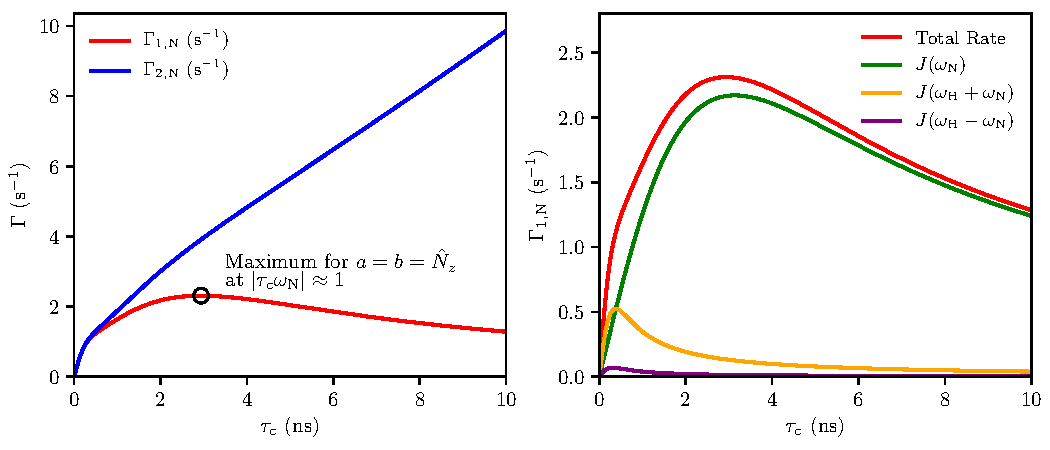
\includegraphics[scale=0.85]{./Figures/SimonsFigs/AppendixBFig.pdf}
\caption{i. Plots of longitudinal ($a = b = \hat{N}_z$) and transverse ($a = b = \hat{N}^+$) nitrogen relaxation rates for an ensemble of $^{15}$N-$^{1}$H spin pairs, whose only relaxation mechanism is the dipolar interaction, undergoing spherical isotropic motion, as a function of $\tau_{\text{c}}$. Parameters used: $B_0 = 11.74 \si{\tesla}$ (corresponding to a $500 \si{\mega \hertz}$ magnet), $\gamma_{\text{H}} = \num{2.675e8} \si{\tesla\per\second}$, $\gamma_{\text{N}} = \num{-2.712e7} \si{\tesla\per\second}$, $r_{\text{NH}} = \num{1.02} \si{\angstrom}$. ii. Plots of the individual contributions to the transverse nitrogen relaxation rate, as a function of $\tau_{\text{c}}$.}
\label{figB.1}
\end{figure}

To gain an appreciation of how the to relaxation rates calculated in sections \ref{secB.2} and \ref{secB.3} vary with rotational correlation time, a $^{15}$N-$^{1}$H dipolar system is considered, in a magnetic field of $\num{11.74} \si{\tesla}$, corresponding to a $\num{500} \si{\mega \hertz}$ magnet. Figure \ref{figB.1} illustrates the nitrogen longitudinal and transverse relaxation rates for such a system. \\
For transverse relaxation, beyond $\tau_{\text{c}} \approx 2 \si{\nano\second}$, there is a linear dependence of rate with $\tau_{\text{c}}$. This is since the $J(0)$ term present in \ref{eqB.7} is dominant for large $\tau_{\text{c}}$ values, and the transverse relaxation rate can conveniently be collapsed to:
\begin{equation}
\Gamma_{2,\text{N}} \approx \frac{d_{\text{IS}}^2 \tau_{\text{c}}}{5}  
\end{equation}
For longitudinal relaxation, no such linear dependence is seen, as there isn't a contribution from $J(0)$. The dominant term in $\Gamma_{1,\text{N}}$, for large $\tau_{\text{c}}$ values is $J(\omega_{\text{N}})$, as this is the term with the smallest associated frequency magnitude. Therefore, a maximum occurs very close to the $\tau_{\text{c}}$ value where $J(\omega_{\text{N}})$ reaches a maximum, i.e. $|\omega_{\text{N}} \tau_{\text{c}}| \approx 1$. The three individual contributions to the expression of $\Gamma_{1,\text{N}}$, expressed in \ref{eqB.5}, are plotted in figure \ref{figB.1}. For each of these contributions, a maximum appears when $|\omega \tau_{c}| = 1$, which yields a spectral density of $\frac{\tau_{\text{c}}}{2}$.
\section{Noteworthy Identities}
The following section provides a list of a number of the identities used in the calculations above
\subsection{Operator Products}
\begin{equation*}
\begin{gathered}
\hat{I}_z \hat{I}^- = -\frac{1}{2} \hat{I}^- \hspace{20pt} \hat{I}^- \hat{I}_z = \frac{1}{2} \hat{I}^- \hspace{20pt} \hat{I}_z \hat{I}^+ = \frac{1}{2} \hat{I}^+ \hspace{20pt} \hat{I}^+ \hat{I}_z = -\frac{1}{2} \hat{I}^+ \\
\hat{I}^+ \hat{I}^- = \frac{1}{2} \hat{E} + \hat{I}_z \hspace{3pt} (= \hat{I}^{\alpha}) \hspace{20pt} \hat{I}^- \hat{I}^+ = \frac{1}{2} \hat{E} - \hat{I}_z \hspace{3pt} (= \hat{I}^{\beta})
\end{gathered}
\end{equation*}
\subsection{Commutators}
\begin{equation*}
\begin{gathered}
\comm{\hat{I}_z}{\hat{I}^+} = \hat{I}_z \hat{I}^+ - \hat{I}^+ \hat{I}_z = \hat{I}^+ \hspace{20pt}
\comm{\hat{I}_z}{\hat{I}^-} = \hat{I}_z \hat{I}^- - \hat{I}^- \hat{I}_z = -\hat{I}^- \\
\comm{\hat{I}^+}{\hat{I}^-} = \hat{I}^+ \hat{I}^- - \hat{I}^- \hat{I}^+ = \hat{I}^{\alpha} - \hat{I}^{\beta} = 2 \hat{I}_z \\
\comm{\hat{I}^+ \hat{S}^+}{\hat{I}^- \hat{S}^-} = \hat{I}^+ \hat{I}^- \hat{S}^+ \hat{S}^- - \hat{I}^- \hat{I}^+ \hat{S}^- \hat{S}^+ = \hat{I}_z + \hat{S}_z \\
\comm{\hat{I}^+ \hat{S}^-}{\hat{I}^- \hat{S}^+} = \hat{I}^+ \hat{I}^- \hat{S}^- \hat{S}^+ - \hat{I}^- \hat{I}^+ \hat{S}^+ \hat{S}^- = \hat{I}_z - \hat{S}_z
\end{gathered}
\end{equation*}
\subsection{Expectation Values}
\begin{align*}
&\bra{\hat{I}_z} \ket{\hat{I}_z} = \expval{\hat{I}_z^2} = \frac{1}{4} \expval{\hat{E}} = \frac{1}{4} \left[\bra{\alpha \alpha} \ket{\alpha \alpha} + \bra{\alpha \beta} \ket{\alpha \beta} + \bra{\beta \alpha} \ket{\beta \alpha} + \bra{\beta \beta} \ket{\beta \beta}\right] \\
&\hspace{41pt}= 1 \\
&\bra{\hat{I}_z} \ket{\hat{I}_z + \hat{S}_z} = \expval{\hat{I}_z^2 + \hat{I}_z \hat{S}_z} = \expval{\frac{1}{4} \hat{E} + \hat{I}_z \hat{S}_z} \\
&\hspace{67pt}= \bigg[\mel{\alpha \alpha}{\frac{1}{4} \hat{E} + \hat{I}_z\hat{S}_z}{\alpha \alpha} + \mel{\alpha \beta}{\frac{1}{4} \hat{E} + \hat{I}_z\hat{S}_z}{\alpha \beta} \\
&\hspace{88pt} + \mel{\beta \alpha}{\frac{1}{4} \hat{E} + \hat{I}_z\hat{S}_z}{\beta \alpha} + \mel{\beta \beta}{\frac{1}{4} \hat{E} + \hat{I}_z\hat{S}_z}{\beta \beta} \bigg] \\
&\hspace{67pt} = \frac{1}{2} \left[\bra{\alpha \alpha} \ket{\alpha \alpha} + \bra{\beta \beta} \ket{\beta \beta}\right] \\
& \hspace{67pt} = 1 \\
&\bra{\hat{I}_z} \ket{\hat{I}^- \hat{S}^+} = -\frac{1}{2}\expval{\hat{I}^- \hat{S}^+} \\
& \hspace{59pt} = -\frac{1}{2} \big[ \mel{\alpha \alpha}{\hat{I}^- \hat{S}^+}{\alpha\alpha} + \mel{\alpha \beta}{\hat{I}^- \hat{S}^+}{\alpha\beta}  \\
& \hspace{95pt} + \mel{\beta \alpha}{\hat{I}^- \hat{S}^+}{\beta\alpha} + \mel{\beta \beta}{\hat{I}^- \hat{S}^+}{\beta\beta} \big] \\
& \hspace{59pt} = -\frac{1}{2} \bra{\beta \alpha} \ket{\alpha \beta} \\
& \hspace{59pt} = 0 \\
&\bra{\hat{I}^+} \ket{\hat{I}^+} = \expval{\hat{I}^- \hat{I}^+} = \expval{\frac{1}{2} \hat{E} - \hat{I}_z} \\
& \hspace{48pt}= \bigg[\mel{\alpha \alpha}{\frac{1}{2} \hat{E} - \hat{I}_z}{\alpha \alpha} + \mel{\alpha \beta}{\frac{1}{2} \hat{E} - \hat{I}_z}{\alpha \beta} \\
&\hspace{69pt} + \mel{\beta \alpha}{\frac{1}{2} \hat{E} - \hat{I}_z}{\beta \alpha} + \mel{\beta \beta}{\frac{1}{2} \hat{E} - \hat{I}_z}{\beta \beta} \bigg] \\
& \hspace{48pt}= \bra{\alpha \alpha} \ket{\alpha \alpha} + \bra{\alpha \beta} \ket{\alpha \beta} \\
& \hspace{48pt} = 2
\end{align*}

\begin{singlespacing}
\printappendixbibliography
\end{singlespacing}
\end{appendixtext}
